\section{Implementation}
\subsection{Class diagram}
\begin{figure}[h!]
\centering
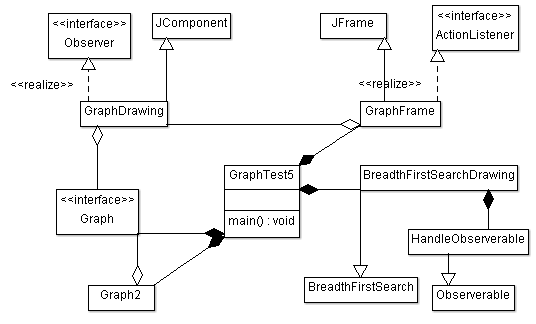
\includegraphics[width=0.5\textwidth]{./images/class_diagram}
\caption{Class diagram of application}
\label{fig:classdiagram}
\end{figure}~\\
The class diagram (figure \ref{fig:classdiagram}) show mainly classes of the functions in program. The \textit{main} method located in the \textit{GraphTest5} class . To present the graph on the GUI, we use \textit{GraphDrawing} and \textit{GraphFrame} class. For the breadth-first search, we have \textit{BreadthFirstSearch} and \textit{BreadthFirstSearchDrawing} class. Final, the edge coloring located in the \textit{Graph2} class. Besides, we also have another classes to support the main classes in the diagram. The detail in the sections below.
\subsection{Represent the graph on the GUI}
Based on the project provided by the supervisor. Program defines the classes to implement the functions of program.
To display the graph on the GUI, vertices and the edges must be have coordinate. By default, vertices represented by the background is yellow, the border is red and the color for label is blue.
\\[0.5cm]
Classes to represent the graph on GUI are:
\begin{itemize}
\item \textbf{VertexCoordinates} (\textit{drawing} package): represent the states with the position.
\item \textbf{DirectedEdgeWithColor} and \textbf{DirectedEdgeWithLabel} (\textit{graph} package): represent the transitions with the label and color.
\item \textbf{GraphDrawing} (\textit{drawing} package): represent the graph
\item \textbf{Drawing} (\textit{drawing} package): support the drawing methods (draw state, transition,...)
\end{itemize}
Our proposal for display the graph on GUI:
\begin{enumerate}
\item Get the number of vertices
\item Calculate the position of each vertex on GUI (based on the layout)
\item Re-create the vertices with the coordinate.
\item Drawing the states
\item Drawing the transition and label
\end{enumerate}
\subsection{The Breadth-first search algorithm}
To implement the breadth-first search algorithm, we have added the classes \textbf{VertexWithAction}, \textbf{BreadthFirstSearch}, \textbf{BreadthFirstSearchDrawing} and added the methods into \textbf{GraphDrawing} class to represent the change when run algorithm.
\\[0.5cm]
Classes defined BFS algorithm are:
\begin{itemize}
\item \textbf{VertexWithAction} (\textit{drawing} package): creates a vertex on the action when algorithm run.
\item \textbf{BreadthFirstSearch} (\textit{util} package): implements the BFS algorithm with two methods that are enqueue and dequeue a vertex.
\item \textbf{BreadthFirstSearchDrawing} (\textit{drawing} package): extends from BreadthFirstSearch. It represents the algorithm step by step.
\item \textbf{GraphDrawing}(the \textbf{update} method): updated the state of vertex when algorithm is running on it.
\end{itemize}
\subsection{The Misra and Gries edge coloring algorithm}
The algorithm indicates the number of color to coloring all the edges of the graph with at most $\Delta(G) + 1$ colours. Based on the set colors of edges, program can add a new color or not. After that, program applied the algorithm to coloring all the edges of the graph.
\\[0.5cm]
Classes implemented the edge coloring algorithm are:
\begin{itemize}
\item The previous classes: represent the graph, edge with coloring.
\item \textbf{Graph2} (\textit{graph} package): implements the algorithm
\end{itemize}
Our proposal for edge coloring:
\begin{enumerate}
\item Get the set color of edges
\item Get the maximal ``fan" \textit{\textless f..l \textgreater} of vertex X
\item Get two colors are free on X (color c) and the vertex latest (color d) in fan of X 
\item Get the cd-path of X
\item Invert the cd-path
\item Find the vertex v in fan such that it remains is fan and color d is free on v
\item Rotate the new fan and coloring the Xv with d
\end{enumerate}